\section{Methodology}
\label{ch:method}
\noindent	

\subsection{IoT scheme}
\label{ch:method:model}
The structure of the IoT system including the planned devices can be found in figure \ref{fig:communication}. 
\begin{figure}[H]
    \centering
    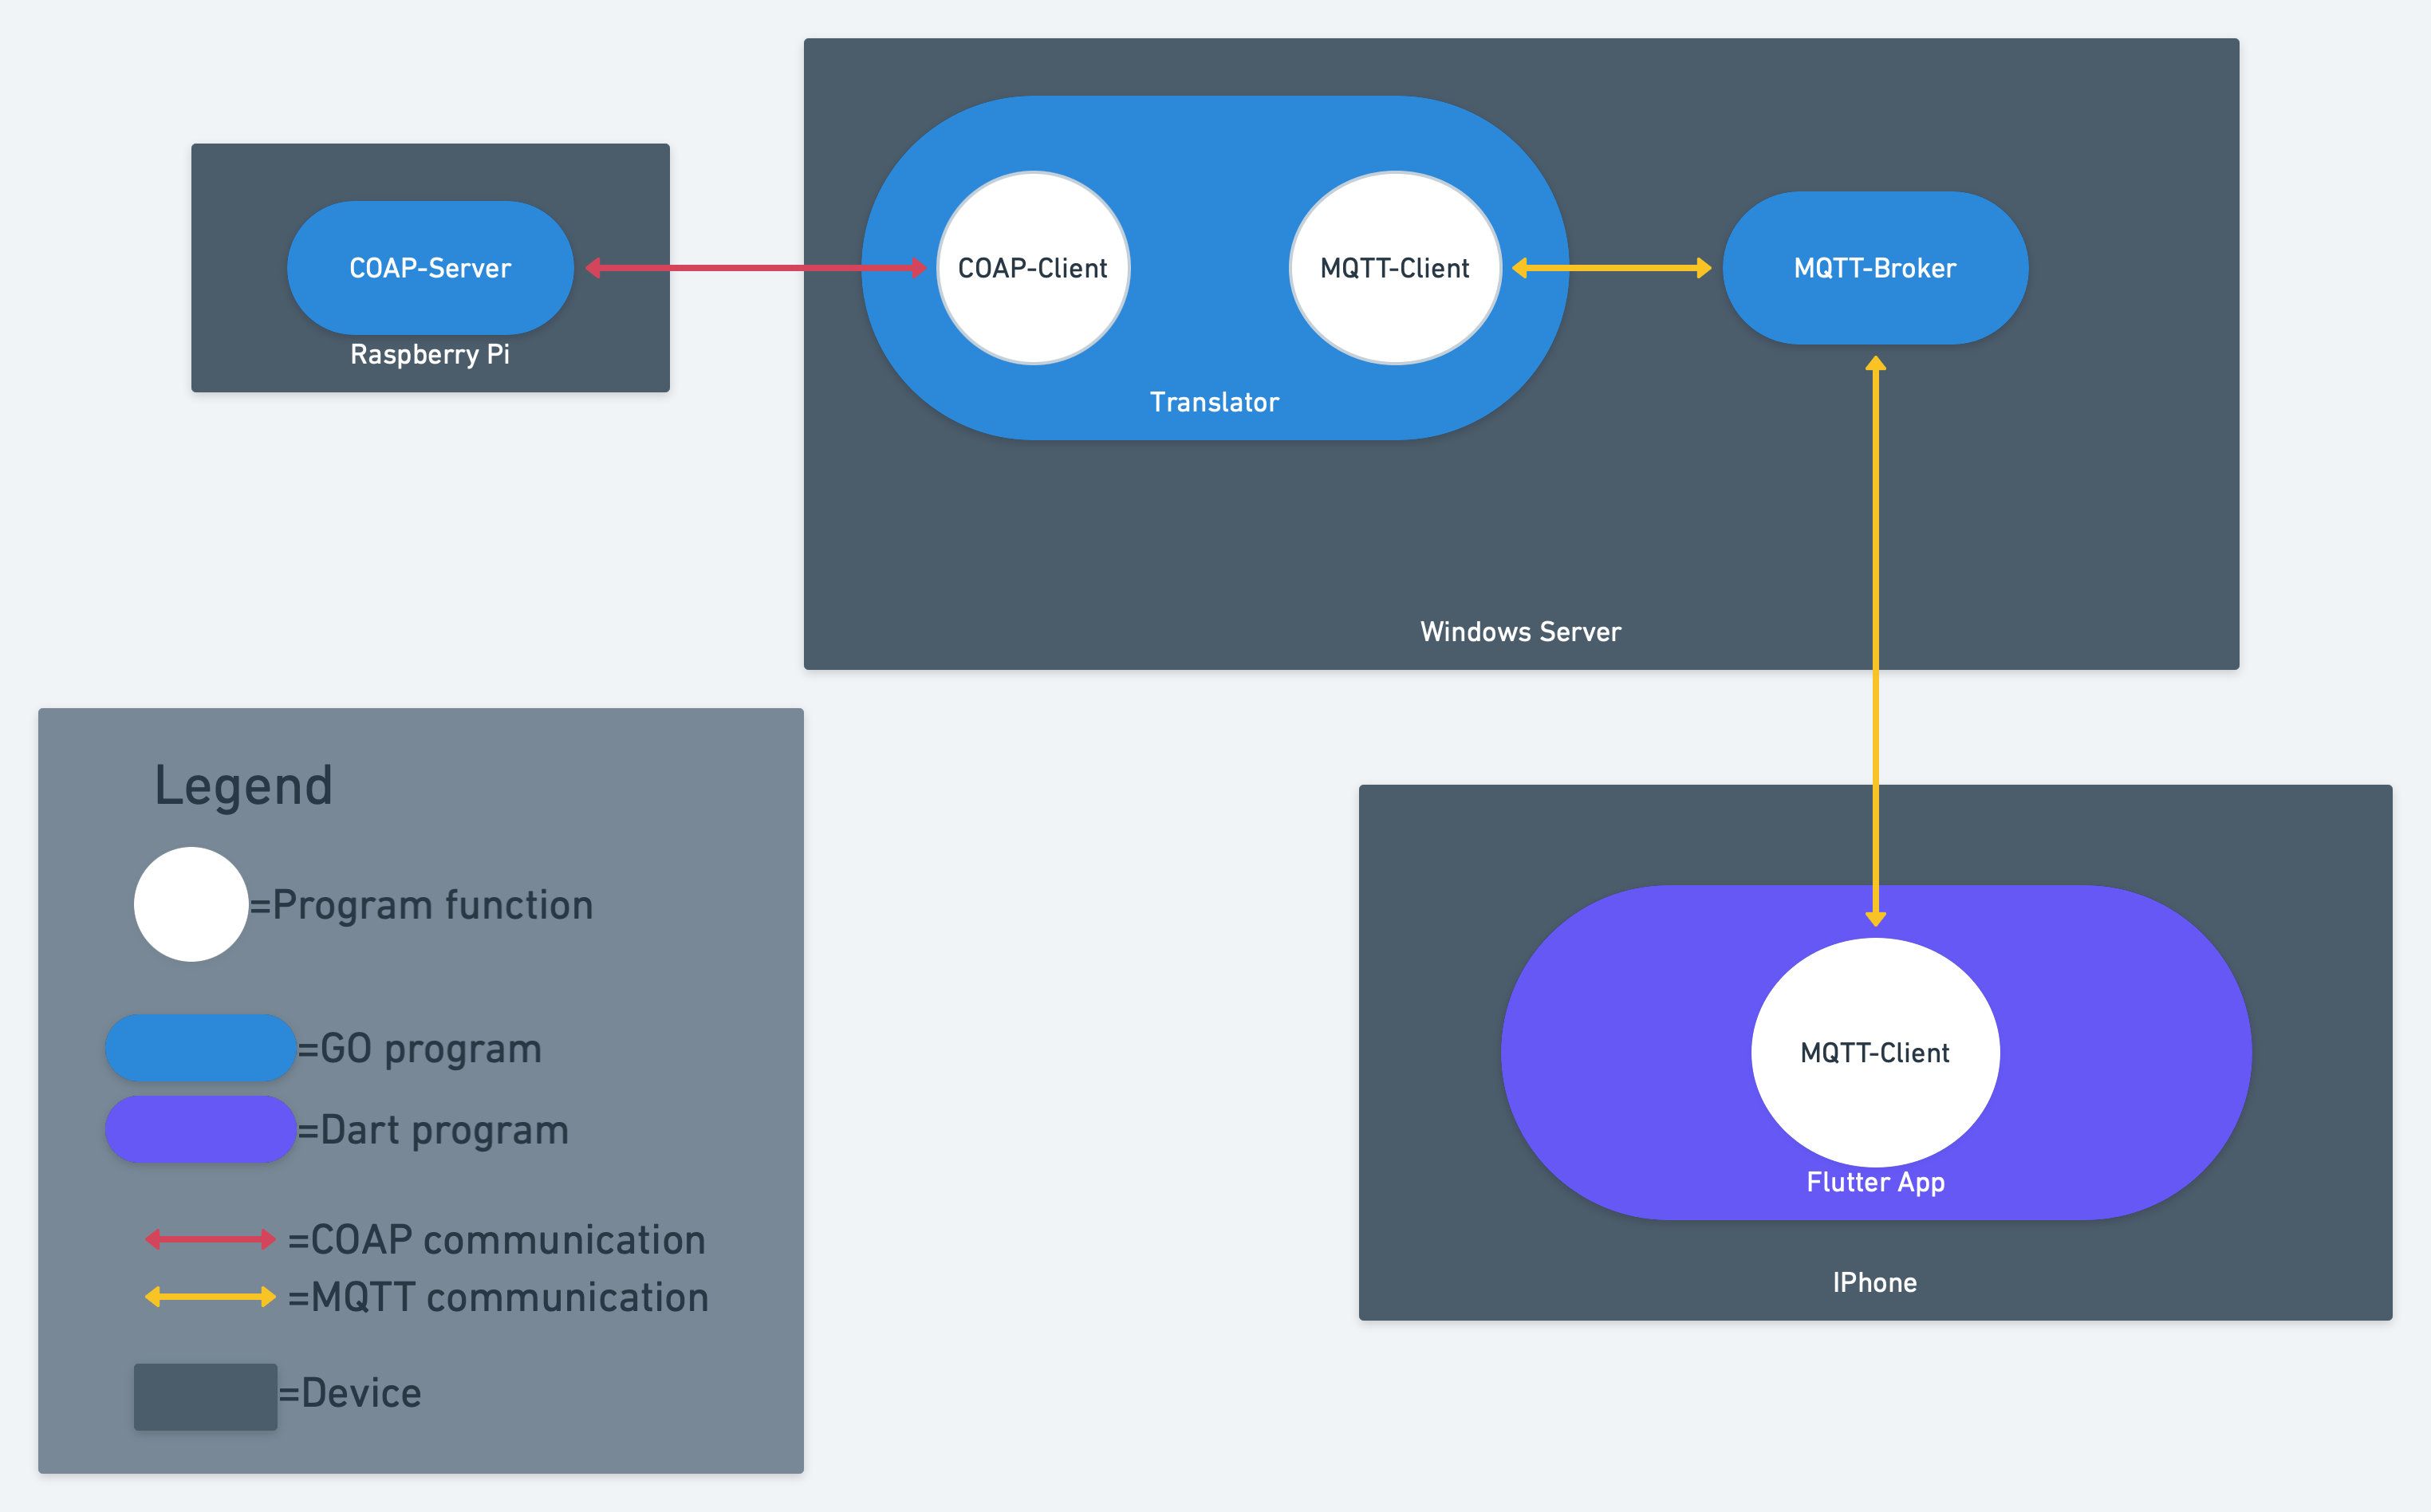
\includegraphics[width=1\textwidth]{img/communication.png} 
    \caption{The planned communication scheme. See legend for explanation}
    \label{fig:communication}
\end{figure}




With regards to C- and D-level diploma work, it is insufficient to merely perform a practical construction or programming project. A systematic study must also be carried out, e.g. an evaluation and analysis of the design or program. The study should result in objective facts, preferably in the form of tables and diagrams, into which your own conclusions are built in. The study can be a verification of a design that meets the requirement specification, or a comparison of competing alternatives. It is acceptable to allow users to answer a questionnaire or be interviewed. It is also possible to evaluate web-pages and other user interfaces according to usability criteria.

The method section is the point at which your chosen method and intended procedure during the research are discussed. This section shall not be a chronological diary filled with irrelevant details, but should contain information given in such a way that it is understandable for the reader and enables him/her to interpret your results and repeat your work, i.e. in order to check the results. Here, the tools, assumptions, mathematical models, performance measures and assessment criteria are presented. It is also at this point that the means adopted for the evaluation and verification of the computer programs and technical solution proposals are presented. This can include a test plan to check that the structure works and criteria to assess its usefulness. In research reports regarding natural science and technology this chapter is often called “Model”, “System Model” or “Simulation Model”.

Justify your choice of methodology/model. This choice is very important, because it could be the actual key to the result of your research. Comment on the method's possible weaknesses and problems that may arise during actual implementation. Refer to the problem wording in the introduction chapter. It is possible, for example, to write “problem P1 is attempted through the method M1 and problem P2 through…” 

In your report, you should - depending on what the report is about- find information about what you have investigated and how you have gathered and processed data. Possible questionnaires, interview questions and the likes can be presented as appendices. Detailed descriptions concerning experimental formats of possible interest to those wanting to repeat the experiment should also be included in this chapter.
